\documentclass[12pt,a4paper]{article}
\usepackage{hyperref}
\usepackage[a4paper]{geometry}

\usepackage{Sweave}
\begin{document}
\Sconcordance{concordance:report.tex:report.Rnw:%
1 4 1 1 0 6 1 1 5 11 1 1 2 1 0 1 1 7 0 1 1 9 0 1 3 5 0 1 2 1 1 1 2 5 0 %
1 2 1 1 1 2 1 0 1 1 7 0 1 1 9 0 1 3 5 0 1 2 1 1 1 2 5 0 1 2 1 1 1 2 5 0 %
1 3 1 0 2 1 9 0 1 4 7 0 1 3 1 0 1 1 7 0 1 5 4 0 1 1 4 0 1 3 1 0 1 1 7 0 %
1 5 4 0 1 1 4 0 1 3 1 0 1 1 7 0 1 4 3 0 1 1 4 0 1 2 1 1 1 2 18 0 1 2 1 %
1 1 2 16 0 1 2 3 1}


\title{Effect of beta and delta/theta frequencies of binaural beats on attention in a neutral and incongruent Stroop task or whatever}
\date{}
\maketitle


\section*{Data processing and reporting tools}

A Ruby script was used to prepare for analysis the raw files returned by the EncephalApp. R was used to automatize the analysis of the data and R integrated with Sweave to build this report. Raw data and all R scripts used in the analysis and the reporting can be found at \url{https://github.com/xdurana/R/tree/master/binaural-beats}.

\section*{Analysis of the reaction time (RT)}

\begin{itemize}

\item[1] Read the file with all the single measures and define the factors. For each group, calculate the descriptive statistics for the dependent variable RT: mean, standard deviation, median and median absolute deviation. A group is defined by a subject, a Stroop level (off, on) and a type of sound (a, b). The data file item.csv can be found at \url{https://github.com/xdurana/R/blob/master/binaural-beats/items.csv}.

\item[2] Plot the histogram, the summary of the data and the QQPlot for each condition.
\begin{Schunk}
\begin{Sinput}
> hist(stroop$time, breaks=200)
> ddply(stroop, .(sound), summarise, mean=mean(time), sd=sd(time))
\end{Sinput}
\begin{Soutput}
  sound     mean        sd
1     a 1.305767 0.4511453
2     b 1.280535 0.4530630
\end{Soutput}
\begin{Sinput}
> ddply(stroop, .(level), summarise, mean=mean(time), sd=sd(time))
\end{Sinput}
\begin{Soutput}
  level     mean        sd
1   off 1.238730 0.3848125
2    on 1.347572 0.5050838
\end{Soutput}
\end{Schunk}
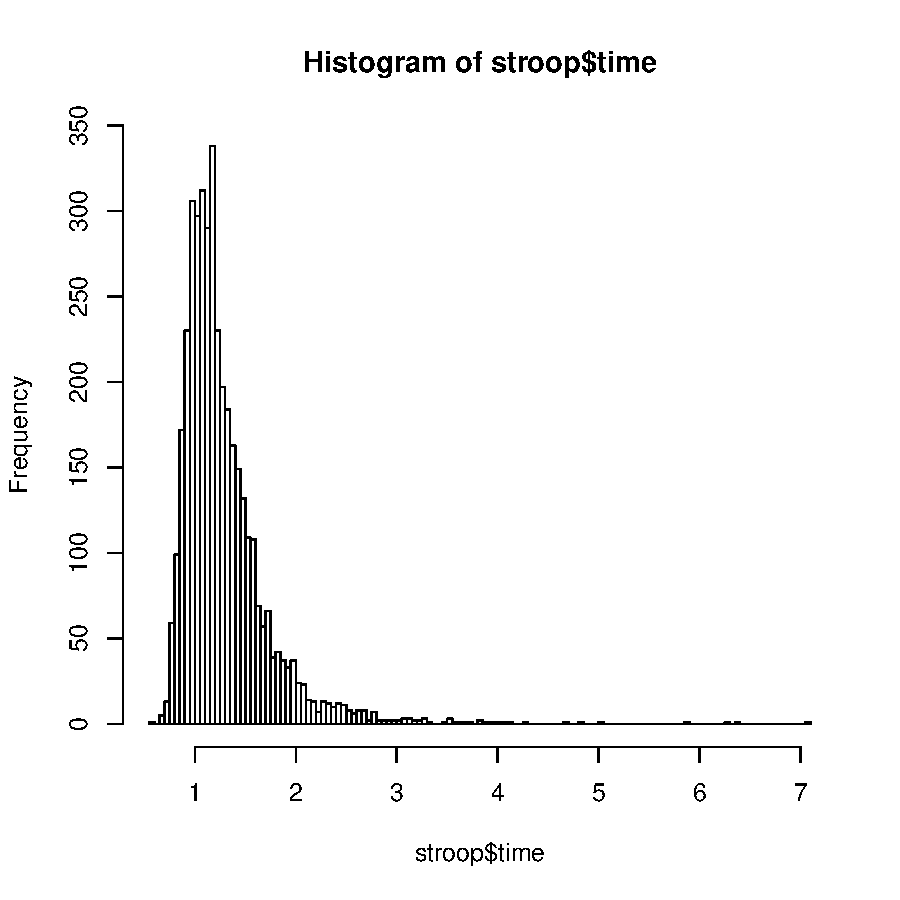
\includegraphics{report-002}
\begin{Schunk}
\begin{Sinput}
> qqmath(~time|level*sound, groups=subject, data=stroop)
\end{Sinput}
\end{Schunk}
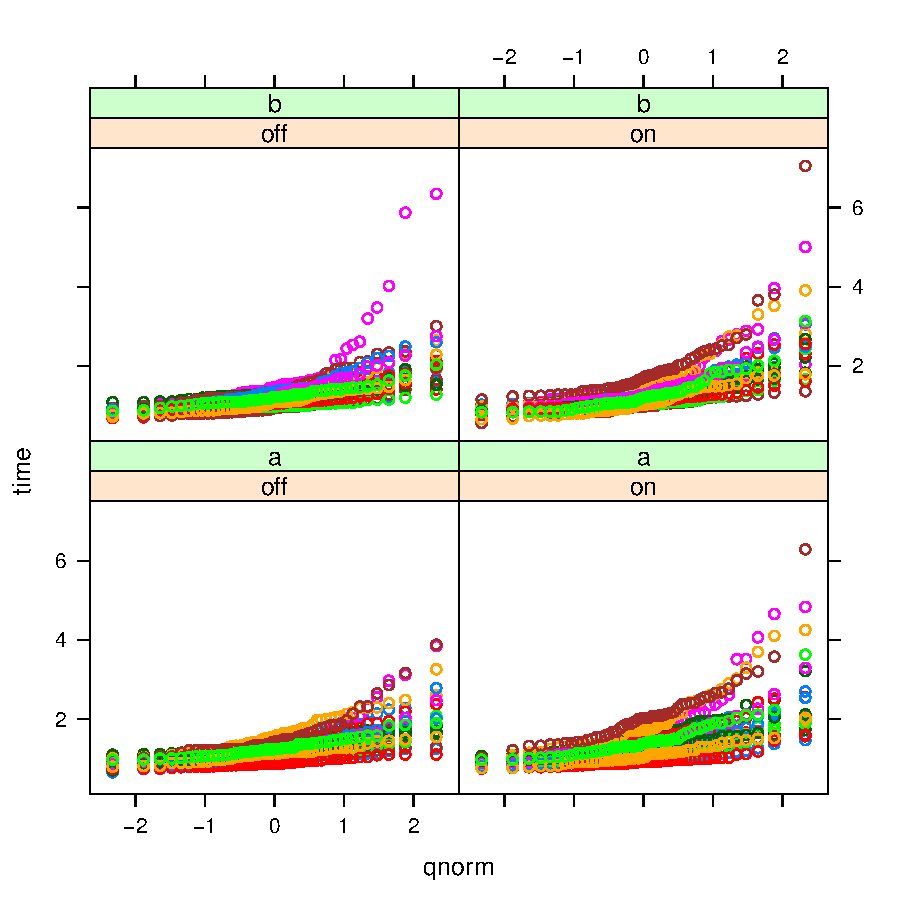
\includegraphics{report-003}

\item[3] Boxplot for each group to see the outliers.
\begin{Schunk}
\begin{Sinput}
> boxplot(stroop$time~stroop$sound+stroop$level+stroop$subject)
\end{Sinput}
\end{Schunk}
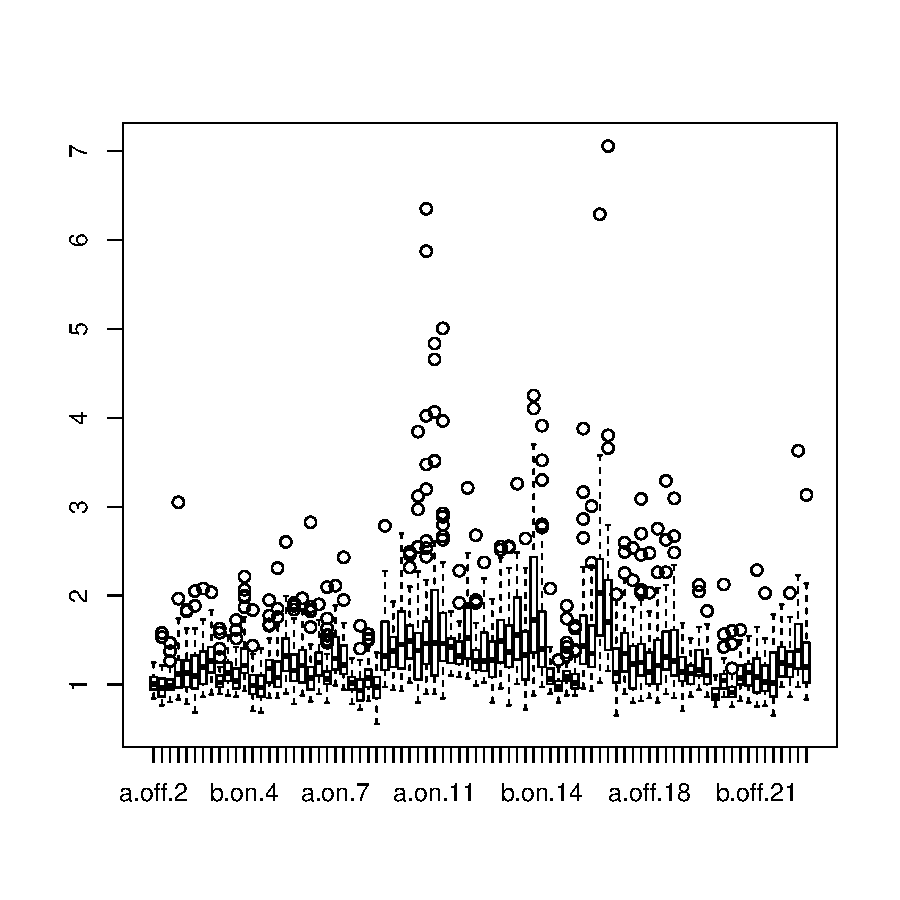
\includegraphics{report-004}

\item[4] Remove the outliers that are beyond the mean + 2*sd of each group, and plot the graphics.
\begin{Schunk}
\begin{Sinput}
> hist(stroop_without_outliers$time, breaks=200)
> ddply(stroop_without_outliers, .(sound), summarise, mean=mean(time), sd=sd(time))
\end{Sinput}
\begin{Soutput}
  sound     mean        sd
1     a 1.263362 0.3617619
2     b 1.229600 0.3344639
\end{Soutput}
\begin{Sinput}
> ddply(stroop_without_outliers, .(level), summarise, mean=mean(time), sd=sd(time))
\end{Sinput}
\begin{Soutput}
  level     mean        sd
1   off 1.198798 0.2917018
2    on 1.294286 0.3920836
\end{Soutput}
\end{Schunk}
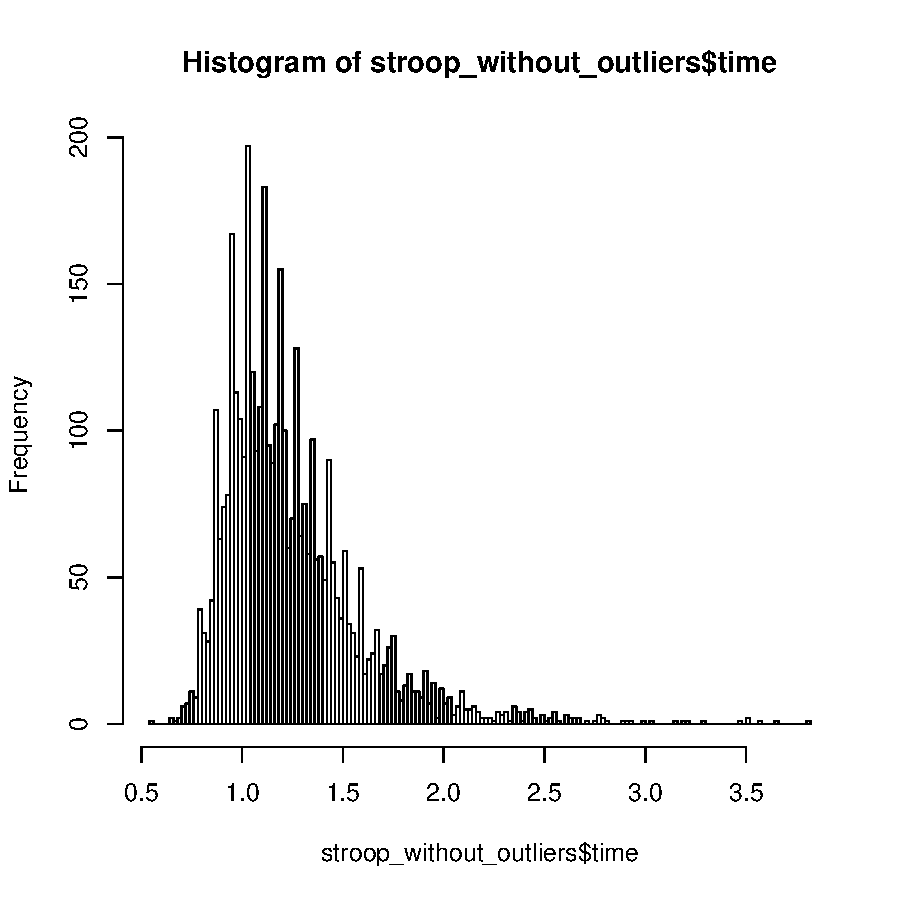
\includegraphics{report-005}
\begin{Schunk}
\begin{Sinput}
> qqmath(~time|level*sound, groups=subject, data=stroop_without_outliers)
\end{Sinput}
\end{Schunk}
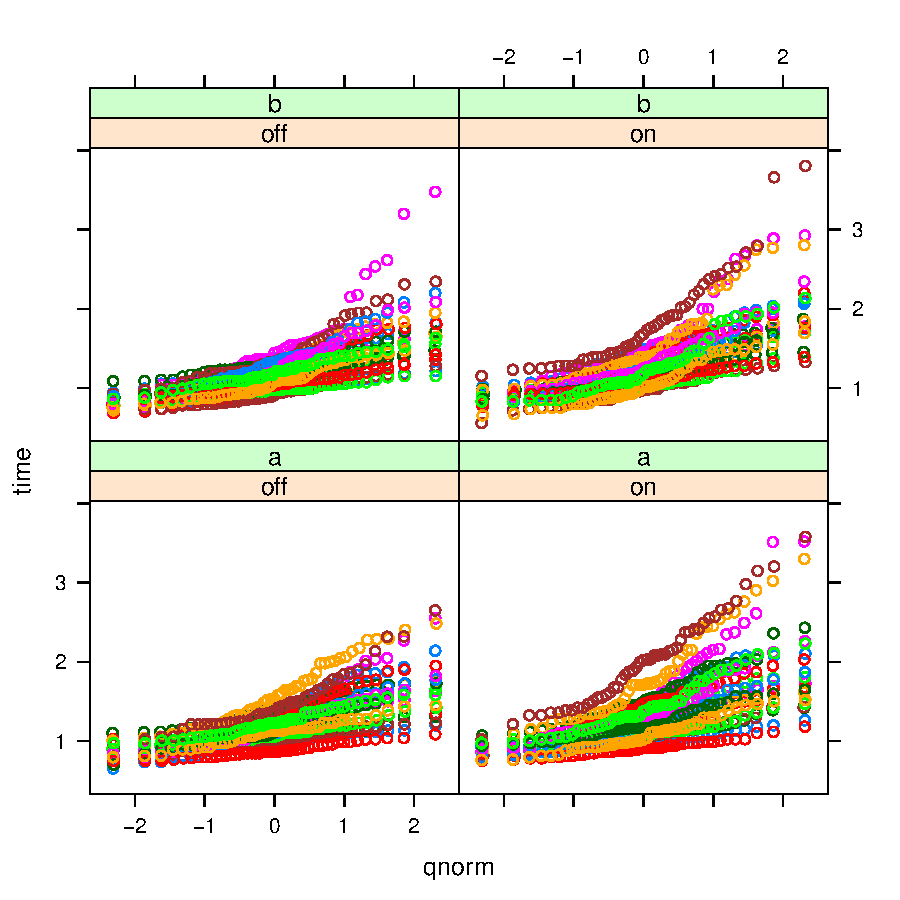
\includegraphics{report-006}

\item[5] Another boxplot for each group.
\begin{Schunk}
\begin{Sinput}
> boxplot(stroop_without_outliers$time~stroop_without_outliers$sound+stroop_without_outliers$level+stroop_without_outliers$subject)
\end{Sinput}
\end{Schunk}
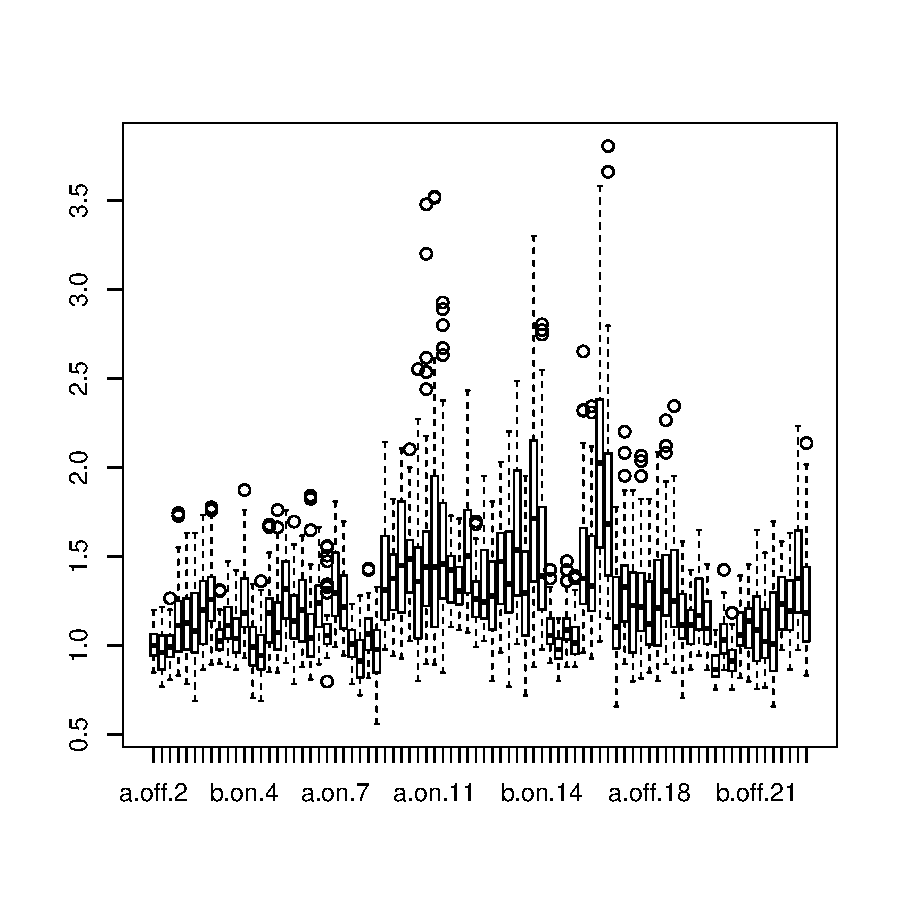
\includegraphics{report-007}

\item[6] Summarize the mean reaction time of each group and plot the boxplots for each level and condition
\begin{Schunk}
\begin{Sinput}
> interaction.plot(summary$level, summary$sound, summary$time)
\end{Sinput}
\end{Schunk}
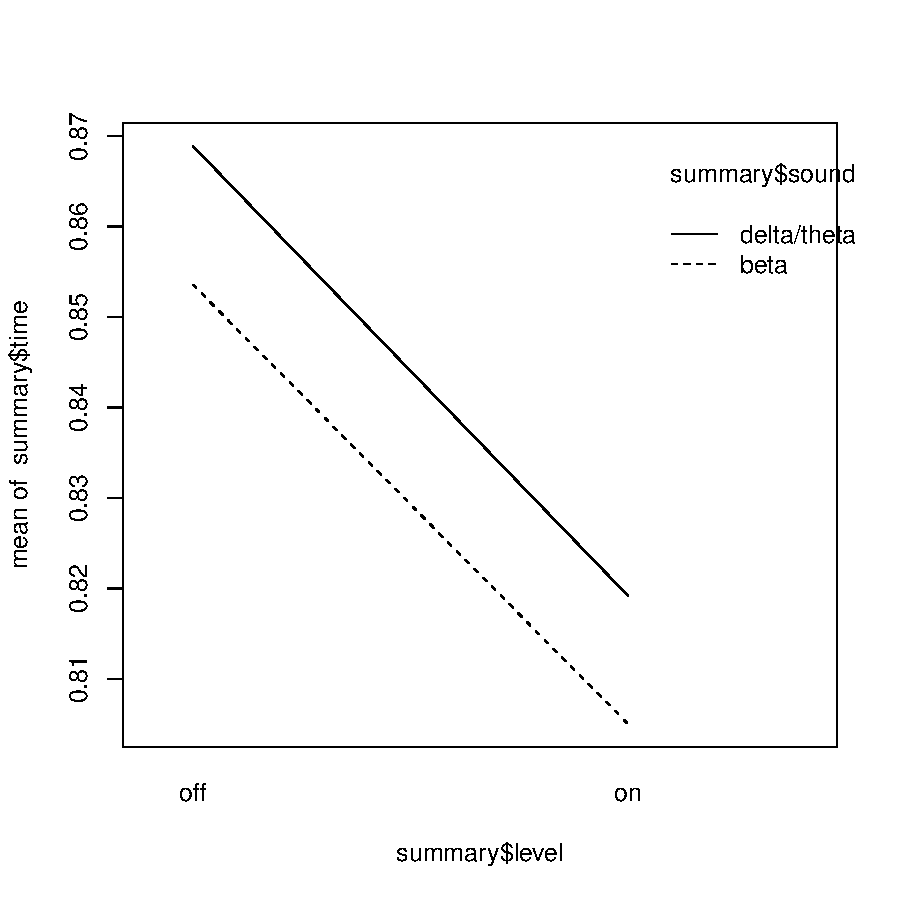
\includegraphics{report-008}
\begin{Schunk}
\begin{Sinput}
> bwplot(time ~ sound | level, data=summary, panel=f.mean, par.settings=bwtheme, layout=c(2,1))
> mean = ddply(summary, .(sound,level), summarise, mean=mean(time))
> ddply(summary, .(sound, level), summarise, mean=mean(time), sd=sd(time))
\end{Sinput}
\begin{Soutput}
        sound level      mean        sd
1        beta   off 0.8535882 0.1223644
2        beta    on 0.8050480 0.1420953
3 delta/theta   off 0.8689046 0.1165105
4 delta/theta    on 0.8192260 0.1185384
\end{Soutput}
\begin{Sinput}
> boxplot(summary$time~summary$sound+summary$level,
+ main = "Reaction time distribution for each condition",
+ xlab = "condition",
+ ylab = "reaction time (s)")
\end{Sinput}
\end{Schunk}
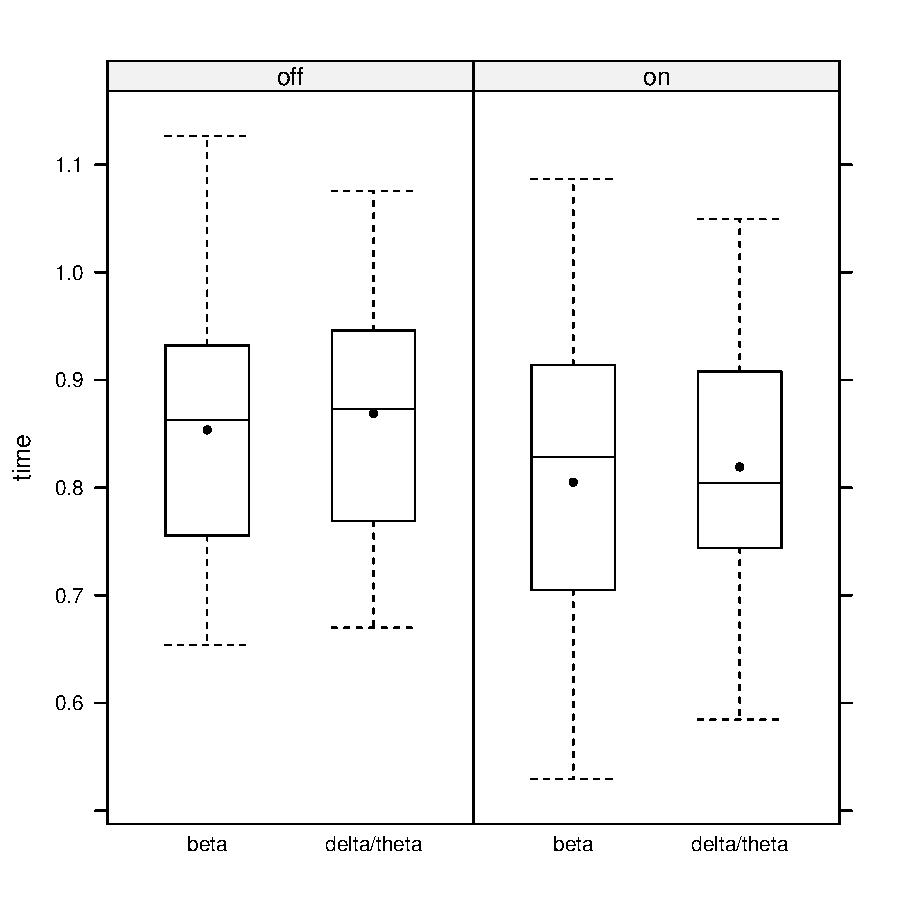
\includegraphics{report-009}
\begin{Schunk}
\begin{Sinput}
> mean = ddply(summary, .(sound), summarise, mean=mean(time))
> ddply(summary, .(sound), summarise, mean=mean(time), sd=sd(time))
\end{Sinput}
\begin{Soutput}
        sound      mean        sd
1        beta 0.8293181 0.1331743
2 delta/theta 0.8440653 0.1187083
\end{Soutput}
\begin{Sinput}
> boxplot(summary$time~summary$sound,
+ main = "Reaction time distribution for each sound",
+ names = c("beta","delta/theta"),
+ xlab = "type of sound",
+ ylab = "reaction time (s)")
> points(mean, pch = 4)
\end{Sinput}
\end{Schunk}
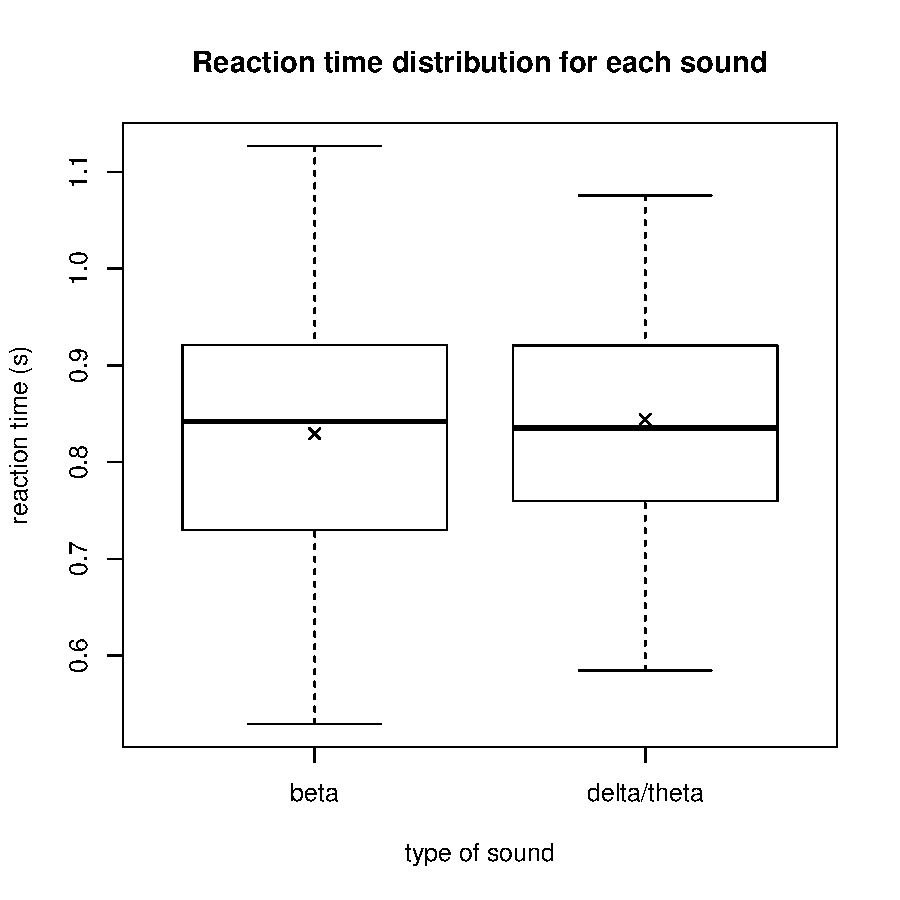
\includegraphics{report-010}
\begin{Schunk}
\begin{Sinput}
> mean = ddply(summary, .(level), summarise, mean=mean(time))
> ddply(summary, .(level), summarise, mean=mean(time), sd=sd(time))
\end{Sinput}
\begin{Soutput}
  level      mean        sd
1   off 0.8612464 0.1181864
2    on 0.8121370 0.1293590
\end{Soutput}
\begin{Sinput}
> boxplot(summary$time~summary$level,
+ main = "Reaction time distribution for each Stroop level",
+ names = c("neutral","incongruent"),
+ xlab = "Stroop level",
+ ylab = "reaction time (s)")
> points(mean, pch = 4)
\end{Sinput}
\end{Schunk}
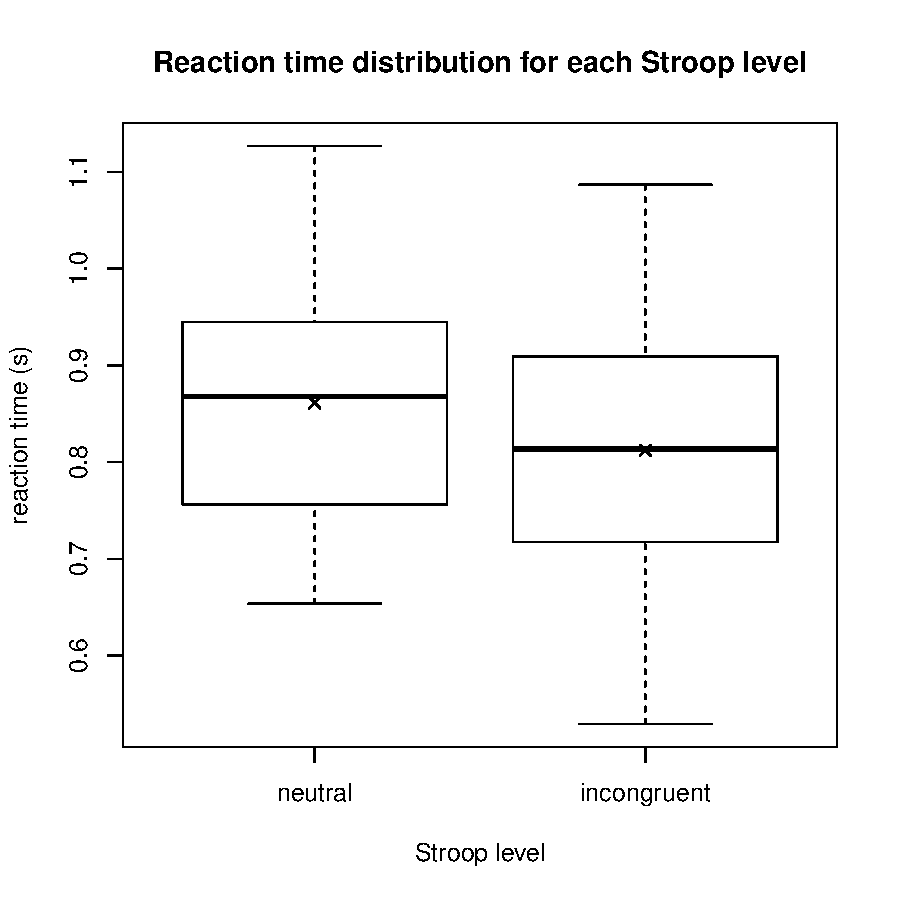
\includegraphics{report-011}
\begin{Schunk}
\begin{Sinput}
> mean = ddply(summary, .(sequence), summarise, mean=mean(time))
> ddply(summary, .(sequence), summarise, mean=mean(time), sd=sd(time))
\end{Sinput}
\begin{Soutput}
  sequence      mean        sd
1       ab 0.8543157 0.1238259
2       ba 0.8190677 0.1263669
\end{Soutput}
\begin{Sinput}
> boxplot(summary$time~summary$sequence,
+ main = "Reaction time distribution for the sequence of sounds",
+ xlab = "Sequence",
+ ylab = "reaction time (s)")
> points(mean, pch = 4)
\end{Sinput}
\end{Schunk}
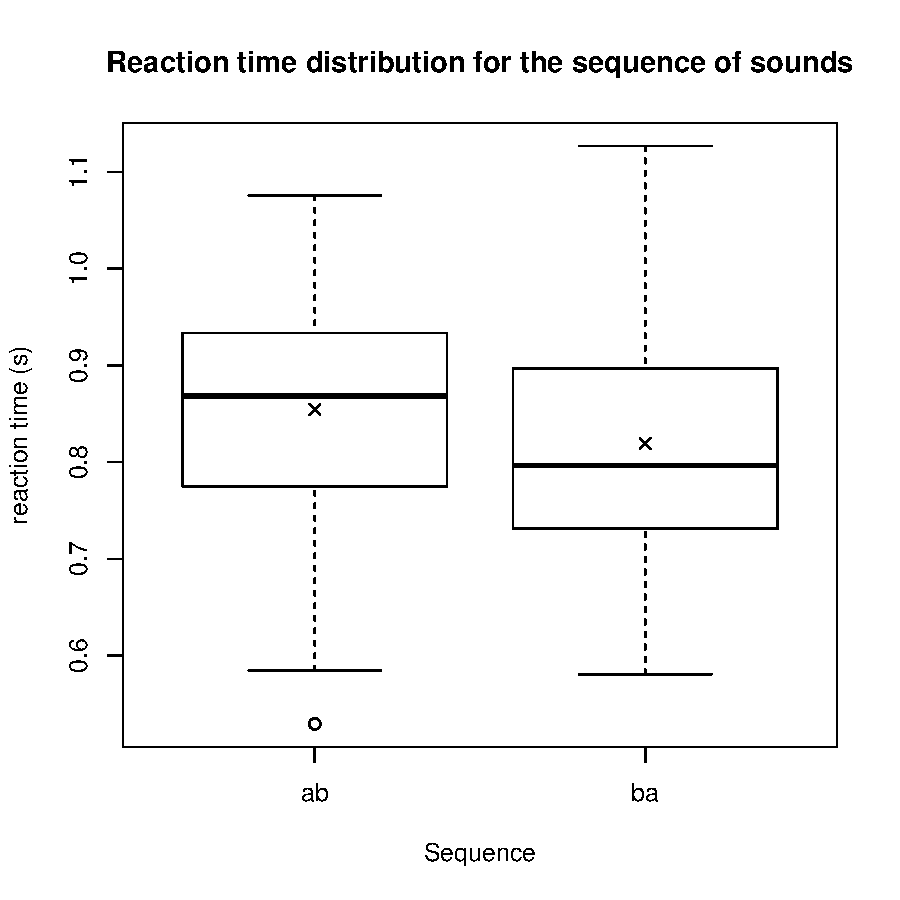
\includegraphics{report-012}

\item[7] Two-way repeated measures ANOVA
\begin{Schunk}
\begin{Sinput}
> print(anova.table, floating=FALSE)
\end{Sinput}
% latex table generated in R 2.15.1 by xtable 1.7-1 package
% Wed Dec 18 21:25:59 2013
\begin{tabular}{lrrrrr}
  \hline
 & Df & Sum Sq & Mean Sq & F value & Pr($>$F) \\ 
  \hline
Residuals & 19 & 1.02 & 0.05 &  &  \\ 
  sound     & 1 & 0.00 & 0.00 & 0.74 & 0.3999 \\ 
  Residuals1 & 19 & 0.11 & 0.01 &  &  \\ 
  level     & 1 & 0.05 & 0.05 & 20.54 & 0.0002 \\ 
  Residuals2 & 19 & 0.04 & 0.00 &  &  \\ 
  sound:level & 1 & 0.00 & 0.00 & 0.01 & 0.9355 \\ 
  Residuals   & 19 & 0.02 & 0.00 &  &  \\ 
   \hline
\end{tabular}\end{Schunk}

\item[8] Post-hoc comparison for the binaural beats
\begin{Schunk}
\begin{Sinput}
> print(test)
\end{Sinput}
\begin{Soutput}
	Paired t-test

data:  mean by sound 
t = -0.8611, df = 19, p-value = 0.3999
alternative hypothesis: true difference in means is not equal to 0 
95 percent confidence interval:
 -0.05059156  0.02109713 
sample estimates:
mean of the differences 
            -0.01474721 
\end{Soutput}
\end{Schunk}

\end{itemize}

\end{document}
